%En-tête classique
\documentclass[11pt,a4paper]{report}
\usepackage[french]{babel}
\usepackage[utf8]{inputenc}
\usepackage[T1]{fontenc}
\usepackage{listings}
\usepackage{subfigure}
\usepackage{xcolor}

%%%% Requis : police Fira Sans + compilation xetex !!! %%%%

%Packages ams
\usepackage[intlimits]{amsmath}
\usepackage{amsfonts}
\usepackage{amssymb}
\usepackage{amsthm}
\usepackage{stmaryrd}

%Fonction indicatrice
\usepackage[upint]{newtxmath}

% réglages font Fira Sans (ATTENTION : XeTex REQUIS !!)
%\usepackage{mathspec}
%\setmainfont[BoldFont=Fira Sans Bold]{Fira Sans}
%\setmathsfont(Digits,Latin)[Numbers={Lining,Proportional}]{Fira Sans}
%\setmathrm[]{Fira Sans}
%\setmathbb[]{Fira Sans Bold}
%\setmonofont[Scale=1]{Ubuntu Mono}

%police perso Fira sans - attention compilation par Latex
\usepackage[default,regular,bold]{sourceserifpro}


%mise en page
\usepackage{multicol}
\usepackage[hidelinks]{hyperref}
\usepackage{fancyhdr}
\usepackage{tabularx} %personalisation des tableaux
\usepackage{graphicx} %importation d'images
\usepackage{enumitem} %personalisation de itemize/enumerate
\usepackage{array} %extension de array/tableaux
\usepackage[left=2cm,right=2cm,top=2cm,bottom=2cm]{geometry} %mise en page
\pagestyle{plain}
\usepackage{lastpage}

%extensions requises par bclogo
\usepackage{xkeyval}
\usepackage{ifthen}
\usepackage{ifpdf}
\usepackage{etoolbox}
\usepackage[tikz]{bclogo}

%paramètres de bclogo
\presetkeys{bclogo}{ombre=true,epOmbre=0.25}{}
\newcommand{\eb}{\end{bclogo}}

%paramétrage bclogo définition
\newcounter{definition}
\setcounter{definition}{0}
\newcommand{\bd}[1]{\addtocounter{definition}{1} \begin{bclogo}[logo=\bcinfo ,sousTitre=#1,nobreak=true]{Définition \thedefinition}}

%paramétrage bclogo théorème
\newcounter{theoreme}
\setcounter{theoreme}{0}
\newcommand{\bt}[1]{\addtocounter{theoreme}{1} \begin{bclogo}[logo=\bctrombone ,arrondi=0.1,sousTitre=#1,nobreak=true]{Théorème \thetheoreme}}

%paramétrage bclogo théorème-définition
\newcounter{deftheo}
\setcounter{deftheo}{0}
\newcommand{\btd}[1]{\addtocounter{deftheo}{1} \begin{bclogo}[logo=\bctrombone ,arrondi=0.1,sousTitre=#1,nobreak=true]{Théorème - Définition \thedeftheo}}

%paramétrage bclogo proposition
\newcounter{proposition}
\setcounter{proposition}{0}
\newcommand{\bp}[1]{\addtocounter{proposition}{1} \begin{bclogo}[logo=\bclampe, sousTitre=#1]{Proposition \theproposition}}

%paramétrage bclogo proposition-définition
\newcommand{\bpd}[1]{\begin{bclogo}[logo=\bctrombone ,arrondi=0.1,sousTitre=#1,nobreak=true]{Proposition - Définition}}

%paramétrage bclogo lemme
\newcounter{lemme}
\setcounter{lemme}{0}
\newcommand{\bl}[1]{\addtocounter{lemme}{1} \begin{bclogo}[logo=\bclampe, sousTitre=#1]{Lemme \thelemme}}

%paramétrage bclogo corollaire
\newcounter{corollaire}
\setcounter{corollaire}{0}
\newcommand{\bcq}[1]{\addtocounter{corollaire}{1} \begin{bclogo}[noborder=true,sousTitre=#1]{Corollaire \thecorollaire}}

%paramétrage bclogo méthode, preuve, remarque, exemple, attention, notations
\newcommand{\bm}[1]{\begin{bclogo}[logo=\bcoutil ,noborder=true,sousTitre=#1]{Méthode}}
\newcommand{\bdm}{\begin{bclogo}[logo=\bcloupe ,margeG=1,noborder=true]{Preuve}}
\newcommand{\br}{\begin{bclogo}[margeG=1,noborder=true,nobreak=true]{Remarque}}
\newcommand{\be}{\begin{bclogo}[margeG=1,noborder=true]{Exemples}}
\newcommand{\bat}{\begin{bclogo}[logo=\bcattention ,margeG=1,noborder=true]{Attention !}}
\newcommand{\bpb}{\begin{bclogo}[logo=\bcattention ,margeG=1,noborder=true]{Problème...}}
\newcommand{\bnot}{\begin{bclogo}[logo=\bccrayon]{Notations}}
\newcommand{\bct}{\begin{bclogo}[logo=\bcbook, noborder=true]{Contexte}}
\newcommand{\bte}{\begin{bclogo}[logo=\bcloupe ,noborder=true,ombre=false]{Tests}}

%texte mathématique en gras
\renewcommand{\textbf}[1]{\begingroup\bfseries\mathversion{bold}#1\endgroup}

%%%raccourcis pour taper et abréviations mathématiques
\newcommand{\bi}{\begin{itemize}}
\newcommand{\ei}{\end{itemize}}
\newcommand{\bn}{\begin{enumerate}}
\newcommand{\en}{\end{enumerate}}
\newcommand{\bpx}{\begin{pmatrix}}
\newcommand{\epx}{\end{pmatrix}}
\newcommand{\ds}{\displaystyle}
\newcommand{\e}{\mathrm{e}}
\newcommand{\R}{\mathbf{R}}
\newcommand{\Z}{\mathbf{Z}}
\newcommand{\N}{\mathbf{N}}
\newcommand{\D}{\mathbf{D}}
\newcommand{\Q}{\mathbf{Q}}
\newcommand{\co}{\mathbf{C}}
\newcommand{\K}{\mathbf{K}}
\newcommand{\ev}{espace vectoriel }
\newcommand{\efini}{Soit $(\Omega, P)$ un espace probabilisé fini}
\newcommand{\sev}{sous-espace vectoriel }
\newcommand{\sevs}{sous-espaces vectoriels }
\newcommand{\kev}{$\K$-espace vectoriel }
\newcommand{\kevs}{$\K$-espaces vectoriels }
\newcommand{\cov}{\mathrm{Cov}}
\newcommand{\vect}{\mathrm{Vect}}
\newcommand{\gl}{\mathrm{GL}}
\newcommand{\tr}{\mathrm{Tr}}
\newcommand{\com}{\mathrm{Com}}
\renewcommand{\phi}{\varphi}
\renewcommand\styleSousTitre[1]{\hfill\textsl{#1}}
\newcommand{\bc}{\begin{cases}}
\newcommand{\ec}{\end{cases}}
\renewcommand{\i}{\mathrm{i}}
\renewcommand{\d}{\mathrm{d}}
\newcommand{\ch}{\mathrm{ch}}
\newcommand{\sh}{\mathrm{sh}}
\renewcommand{\th}{\mathrm{th}}
\newcommand{\non}[1]{\textrm{non}(#1)}
\newcommand{\impq}{\Longrightarrow}
\renewcommand{\Re}{\mathrm{Re}}
\renewcommand{\Im}{\mathrm{Im}}
\newcommand{\card}{\mathrm{Card}}
\renewcommand{\epsilon}{\varepsilon}
\newcommand{\spe}{\mathrm{Sp}}
\renewcommand{\ker}{\mathrm{Ker}}
\newcommand{\rg}{\mathrm{rg}}
\newcommand{\cond}{\mathrm{Cond}}
\newcommand{\ord}{\mathrm{Ord}}
\newcommand{\indic}{\vmathbb{1}}

%abréviations suites (variable n)
\newcommand{\un}[1]{(u_n)_{n\in #1}}
\newcommand{\vn}[1]{(v_n)_{n\in #1}}
\newcommand{\wn}[1]{(w_n)_{n\in #1}}
%limites (variable x par défaut)
\newcommand{\tend}[2][x]{\underset{#1 \to #2}{\longrightarrow}}
\newcommand{\pinf}{+\infty}
\newcommand{\minf}{-\infty}
\newcommand{\Db}{\overline{D}}
\newcommand{\Rb}{\overline{\R}}
%%% %charge fichier des commandes perso

%En-tete et pied de page
\lhead{}
\chead{}
\rhead{}
\lfoot{}
\cfoot{\thepage}

% espace entre chaque paragraphe
\parskip=5pt

\begin{document}
\begin{titlepage}
\vspace*{\fill}
\hrule ~\vspace{0.5cm}

\begin{huge}
\noindent \textbf{Rapport final IEN - groupe 9}
\end{huge} 
\vspace{0.5cm}

\noindent {\Large \textit{Comparaison d'outils de visioconférence sur le plan environnemental}}
\vspace{2cm}

\begin{Large}
\noindent Damien LU, Romain LOIRS, Florian LECOMTE
\end{Large} \\ \\
\begin{Large}
\today
\end{Large}
~\vspace{0.5cm}
\hrule
\vspace*{\fill}
\end{titlepage}

\lstset{basicstyle=\ttfamily,showstringspaces=false,breaklines=true, language=Caml,keywordstyle=\color{blue},commentstyle=\color{gray},breakindent=1.5em,
xleftmargin=2em,xrightmargin=2em,frame=single,rulecolor=\color{orange},
backgroundcolor=\color{yellow!5},columns=fullflexible}
\tableofcontents

\newpage
\chapter*{Introduction}
\addcontentsline{toc}{chapter}{Introduction}

\section{Motivations}
Le contexte actuel lié à la crise du coronavirus favorise le télétravail et augmente mécaniquement l’usage d’outils de collaboration en ligne, en particulier les outils de visioconférence, ce qui amène à une pression sur le réseau et plus particulièrement à une charge importante sur les serveurs de chaque solution. Il est donc important d’un point de vue efficience mais aussi impact environnemental de choisir la solution la plus sobre en ressources. Nous allons nous inspirer de travaux réalisés par l'UTC et d'une étude de Greenspector afin d'analyser d'analyser differents outils de vidéoconférence.

%\section{Résumé des travaux de l'UTC et Greenspector}
\section{Le rapport de l'UTC}
Tout d'abord, l'UTC suppose directement que l'audio et la vidéo sont actifs ; ils considèrent l'impact matériel, logiciel et transport.

Il y a 3 scénarios, tous avec 5 participants : 
\bi \item le premier où la réunion est en présentiel, et chaque membre s'y rend physiquement selon son temps de trajet,
\item le deuxième où la réunion est organisée avec du matériel professionnel pour visioconférence dans l'entreprise à deux endroits, plus un troisième endroit où il y a juste un PC d'un participant, en utilisant la solution Skype,
\item enfin le dernier où les participants se regroupent à 3 endroits différents, donc 3 ordinateurs pour 5 participants, avec de faibles temps de transport et en visioconférence sur Jitsi. \ei

D'après leurs études, le scénario C semble être le moins impactant des 3, sur l'environnement mais aussi sur la santé des participants. On remarque que les logiciels n'ont pas réellement d'impact comparé au matériel utilisé. Ils ont enfin aggravé certains scénarios, mais cela ne changeait pas le constat final. On comprend donc que leur étude n'était pas centrée sur le logiciel utilisé, mais sur ce qu'utilisaient en général les participants.

\section{Le travail de Greenspector}
Greenspector s'intéresse spécifiquement aux différents logiciels de visioconférence. Il y a là encore 3 scénarios, avec cette fois 2 participants : un avec audio, un avec audio + vidéo et enfin un avec audio + vidéo + partage d'écran.

Ils s'intéressent à la quantité de données échangées ainsi qu'à la consommation éléctrique, qu'ils transposent ensuite en équivalent carbone. La conclusion de leurs travaux est que la vidéo consomme énormement, et le partage d'écran moins que la vidéo mais toujours plus que l'audio.

La partie qui consomme le plus est le réseau, mais la consommation de l'appareil est également importante (presque 1 tier). La consommation serveur est très faible. Selon eux l'application qui a le moins d'impact est GoToMeeting, celle qui consomme le plus est Jitsi.

\chapter{Cadre de notre étude}
\section{Objectifs}
L'objectif est de comparer les outils de visioconférence Openmeetings, Zoom et Jitsi dans différentes conditions d'utilisation qui reflètent un usage standard en entreprise ou à l'école. Pour Zoom, nous utiliserons à la fois l'application pour pc et la version web. Pour Openmeetings, nous utiliserons les serveurs dédiés disponible sur le web. Pour Jitsi, nous avons mis en place un serveur de visioconférence Jitsi hébergé par nos soins. Nous utiliserons également les serveurs dédiés sur le web.

\begin{figure}[h]
\begin{subfigure}
  \centering
  
\includegraphics[width=.3\linewidth]{zoom-logo (1).png}
  %\caption{}
  %\label{fig:fig_hist_trans}
\end{subfigure}
\begin{subfigure}
  \centering
  
\includegraphics[width=.3\linewidth]{logo.png}
  %\caption{}
  %\label{fig:fig_hist_trans}
\end{subfigure}
\begin{subfigure}
  \centering
  
\includegraphics[width=.3\linewidth]{logo-jitsi-meet.png}
  %\caption{}
  %\label{fig:fig_hist_trans}
\end{subfigure}
\caption{Logo des différentes applications de visioconférence}
\label{fig:logos}
\end{figure}

Pour chacune de ces applications, nous avons mesuré :
\bi \item la consommation d’énergie des pc lorsque l'application fonctione (Wh),
\item la quantité de données échangées entre le serveur et l'application de visio-conférence (Mo)
\item la projection des données mesurées en impact Carbone (gEqCO2)
\ei

Nous avons également réalisé des tests d'une durée de 30 minutes à travers différents scénarios:
\bi \item conférence simple à trois personnes sans partage audio ni vidéo ni partage d'écran 
\item conférence à trois personnes avec partage audio des trois personnes, sans partage vidéo ni partage d'écran
\item conférence à trois personnes avec partage vidéo et audio mais sans partage d'écran
\item conférence à trois personnes avec partages vidéos, audio et patage écran \ei 

\section{Matériel}
\subsection{Client}
Pour prendre les mesures, nous considérerons un ordinateur portable Acer tournant sous Arch Linux Gnome (voir figure \ref{fig:test}) Pour chacun des scénarios, les mesures sont faites avec uniquement l'application ouverte et sur batterie, ceci pour refléter un usage normal scolaire ou en entreprise.
\begin{figure}[!h]
    \centering
    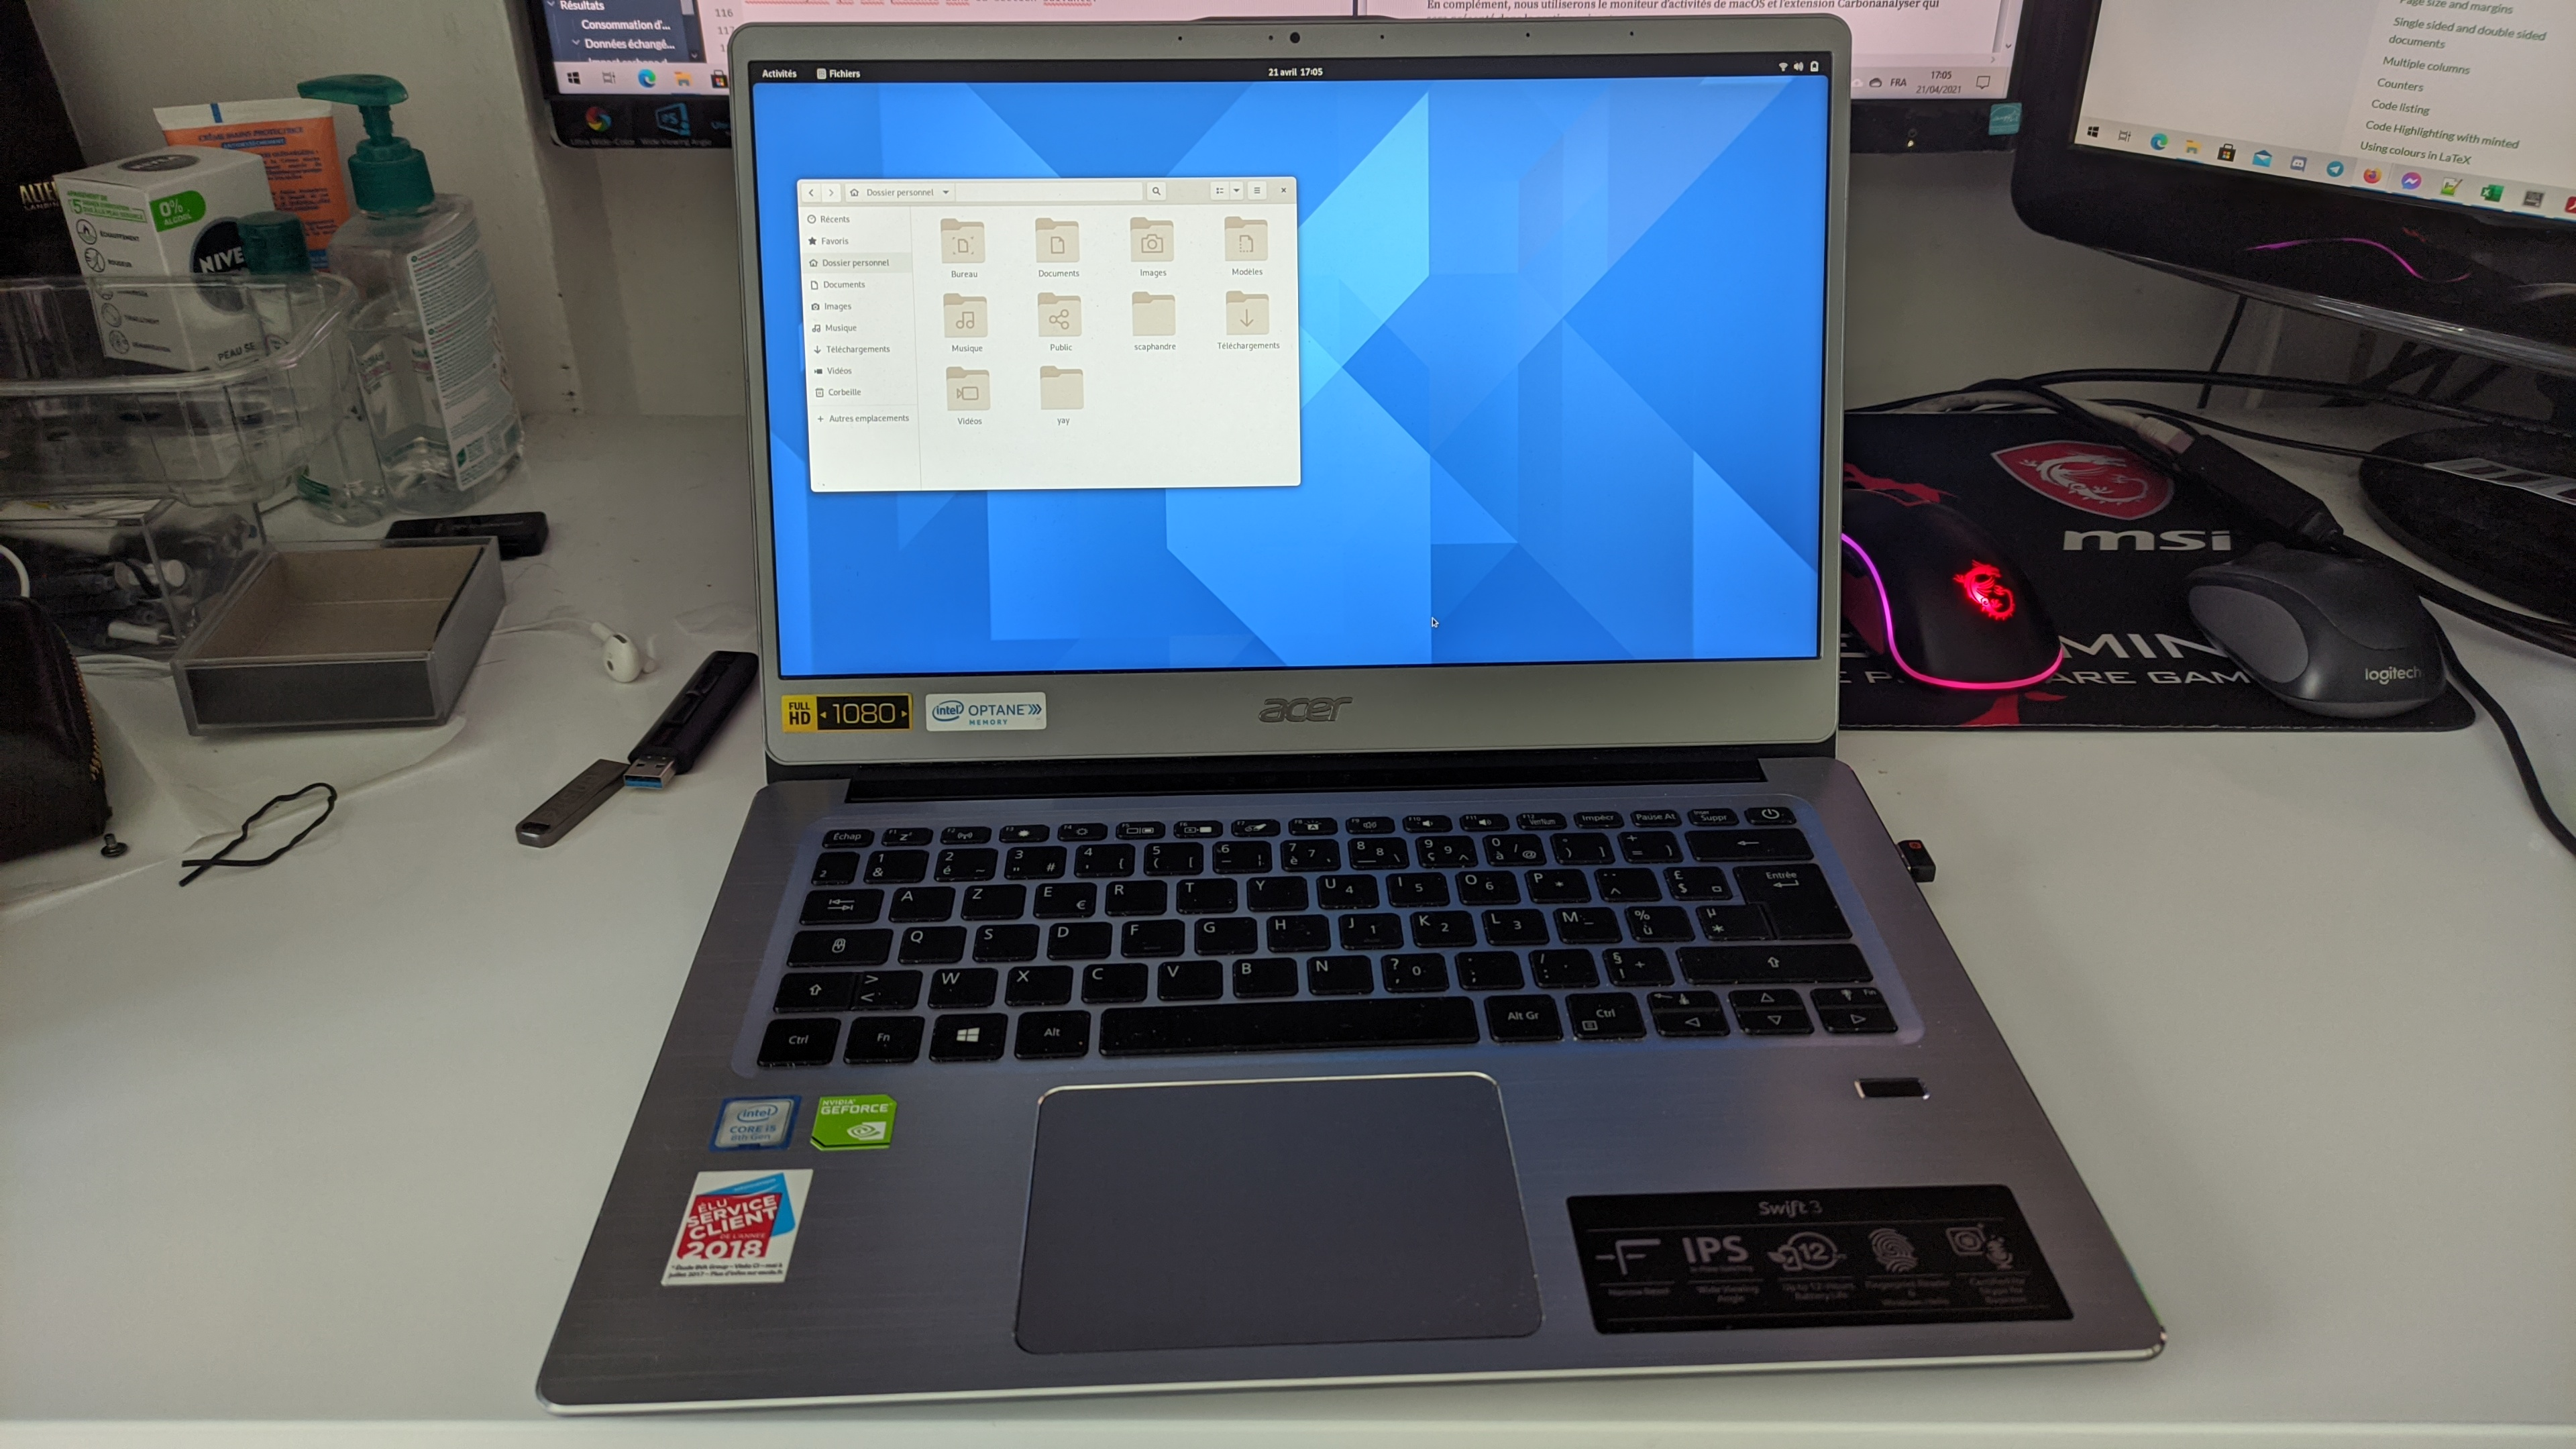
\includegraphics[scale=0.1]{ordinateur.jpg}
    \caption{Ordinateur portable de test}
     \label{fig:test}
\end{figure}
\subsection{Serveur Jitsi}
Une instance de Jitsi a été configurée et hébergée par nos soins (chez Damien) sur un autre ordinateur portable de test. Cette instance est alors accessible avec le lien suivant : \url{https://visio.dlu02.ovh}. Sur ce serveur peuvent alors être mesurées les valeurs de puissance instantanée ainsi que de quantité de données échangée (via les utilitaires présentés à la section suivante), ce qui permet d'avoir un aperçu des ressources utilisées par un serveur de visioconférence. 
\br Le serveur étant un ordinateur portable, qui par définition consomme moins qu'un ordinateur de bureau, et accessoirement encore moins qu'une armoire de serveurs, les valeurs obtenues du côté serveur sont logiquement très inférieures aux valeurs attendues. \eb


\section{Outils de mesures}


\subsection{Carbonanalyser}
L’extension de navigateur Carbonalyser permet de visualiser la consommation électrique et les émissions de gaz à effet de serre (GES) associées à une navigation internet.
Carbonanalyser utilise le modèle "1byte" pour les mesures de consommation électrique. Il s'agit d'un modèle mis au point par The Shift Project dans le cadre du rapport « Lean ICT – Pour une sobriété numérique », publié en octobre 2018. Ce modèle permet de calculer la consommation électrique engendrée par le transfert d’une quantité de données définie, en prenant en compte les consommations associées à la sollicitation :
\bi \item Des centres de données où résident et transitent les données,
\item Des infrastructures réseaux,
\item Du terminal utilisé pour visualiser ou consommer les données. \ei
Deux principales hypothèses sont prises dans la version du modèle "1byte" utilisée dans les calculs de l’add-on :
\bi \item Terminal considéré : une moyenne a été effectuée sur les consommations électriques du smartphone et de l’ordinateur portable ;
\item Réseau considéré : est considéré ici la consommation associée au réseau WIFI.  \ei

La consommation électrique calculée est traduite en émissions de gaz à effet de serre à partir du facteur d’émission de la zone géographique sélectionnée. Le facteur d’émission traduit l’intensité carbone de la production d’électricité, au vu du mix électrique en vigueur dans la zone géographique :
\bi \item Union Européenne : 0,276 kgCO2e/kWh
\item France : 0,035 kgCO2e/kWh
\item Etats-Unis : 0,493 kgCO2e/kWh
\item Chine : 0,681 kgCO2e/kWh
\item Autres (correspond au facteur moyen mondial) : 0,519 kgCO2e/kWh \ei
\bd{Mix électrique} Le mix électrique désigne les sources d’énergie utilisées dans la production d’électricité d’un pays. Leur utilisation se fait en proportions différentes. \eb

\subsection{Moniteur système Gnome}
Pour mesurer les quantités de données, nous utiliserons le moniteur système intégré à Gnome, qui présente le débit de données échangés en temps réel sous forme de graphique (voir figure \ref{fig:gnome}).

\begin{figure}[!h]
    \centering
    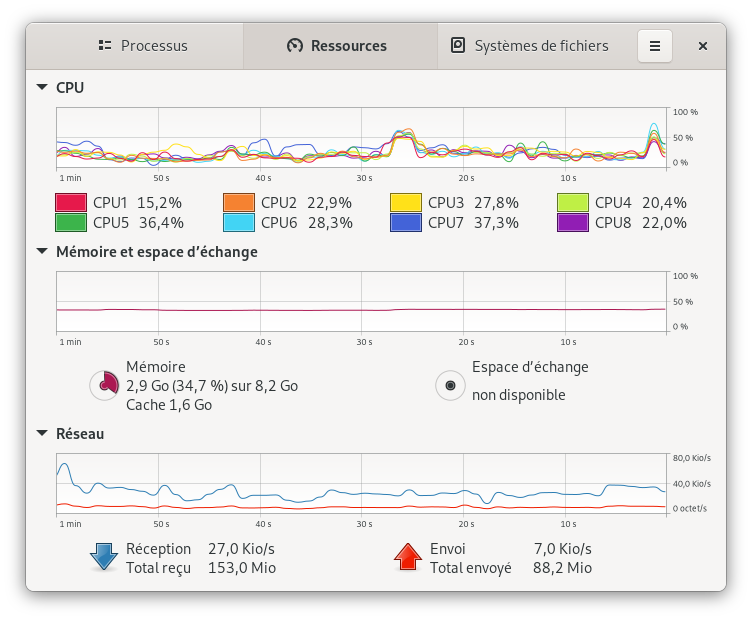
\includegraphics[scale=0.3]{capture_moniteur_sys.png}
    \caption{Moniteur système Gnome et graphique du débit échangé}
     \label{fig:gnome}
\end{figure}

La valeur retenue à l'issue de chaque mesure est la valeur moyenne du débit, et donc pour obtenir la quantité de données échangées, il suffit de multiplier par la durée de la mesure (30 min).

\subsection{iptables}
Pour mesurer la quantité de données échangées en Mo du côté serveur (qui ne possède pas d'interface graphique), nous utiliserons le pare-feu logiciel du serveur \texttt{iptables} qui permet de mesurer la taille totale des paquets correspondant à chaque règle du pare-feu (et donc une règle du pare-feu autorise les échanges entre Jitsi et Internet), comme montré à la figure \ref{fig:iptables}.
\begin{figure}[!h]
    \centering
    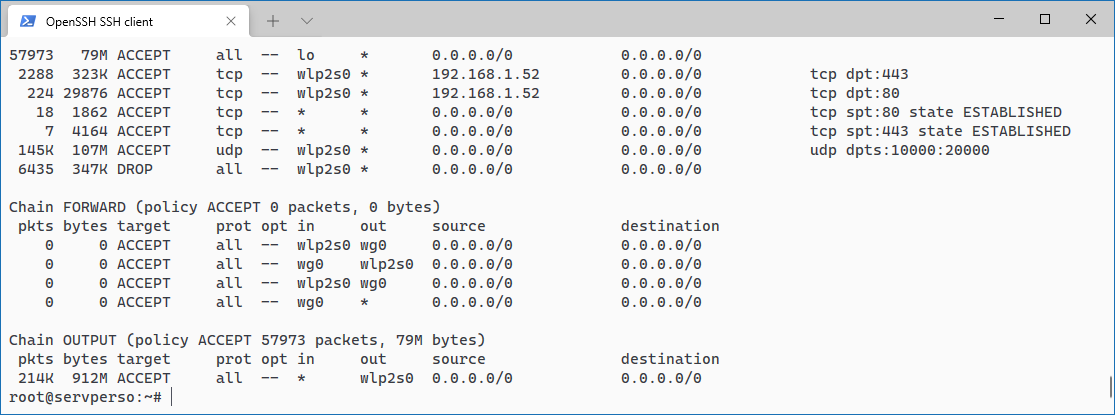
\includegraphics[scale=0.5]{iptables.PNG}
    \caption{Règles du pare-feu iptables et quantité de données échangées}
    \label{fig:iptables}
\end{figure}

Dans notre cas, la règle pour autoriser Jitsi est l'ouverture des ports UDP 10000 à 20000. Ainsi, la taille des paquets reçus indique la quantité de données échangée lors d'une visioconférence.


\subsection{Scaphandre}
Scaphandre est  un logiciel open-source de mesure de la consommation d'énergie d’un serveur informatique ou d'un ordinateur, mais aussi plus précisément des services et applications qu’il exécute. Plus précisément, scaphandre est à la fois un outil utilisable en ligne de commande et un démon (service).
Le projet a notamment pour objectif de rendre la mesure de consommation d'énergie suffisamment simple pour que ça devienne “un basique”, au même titre que le nombre de requêtes par seconde ou la latence, le temps CPU consommé ou la RAM, etc…

Nous utilisons Scaphandre sur la machine cliente pour mesurer la consommation électrique soit du client Zoom, soit du navigateur web, comme montré à la figure \ref{fig:scaph} :
\begin{figure}[!h]
    \centering
    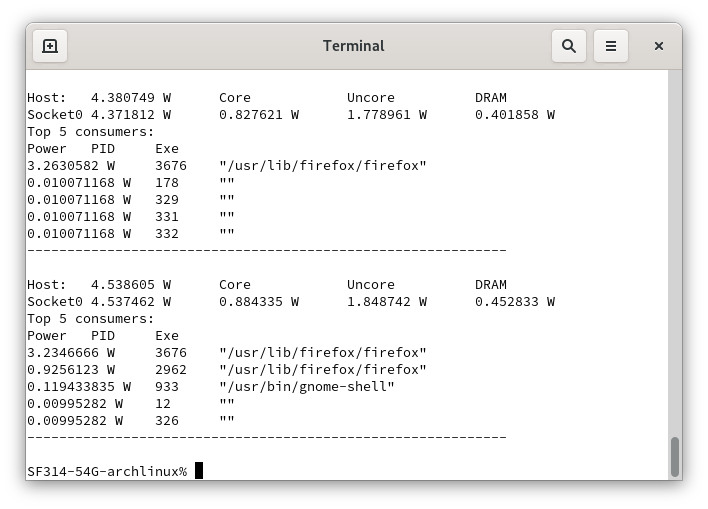
\includegraphics[scale=0.5]{capture_scaphandre.png}
    \caption{Commande \texttt{scaphandre stdout} renvoyant les 5 processus les plus gourmands}
    \label{fig:scaph}
\end{figure}



\chapter{Résultats}

\section{Consommation d’énergie des applications de visioconférence}

\paragraph{}
Dans ce qui suit, nous allons nous intéréssser à la consommation énergétique des applications de visioconférence sur l'ordinateur de l'utilisateur. Les résultats sont présentés sur la figure \ref{fig:graph_energie}. Rappelons également que ces valeurs sont données pour une minute de visioconférence à 3 participants (mesure de 30 minutes normalisée à 1 minute). Plus la consommation est faible, plus l'impact environnemental de l'applcation est faible.


\begin{figure}[h]
  \centering
  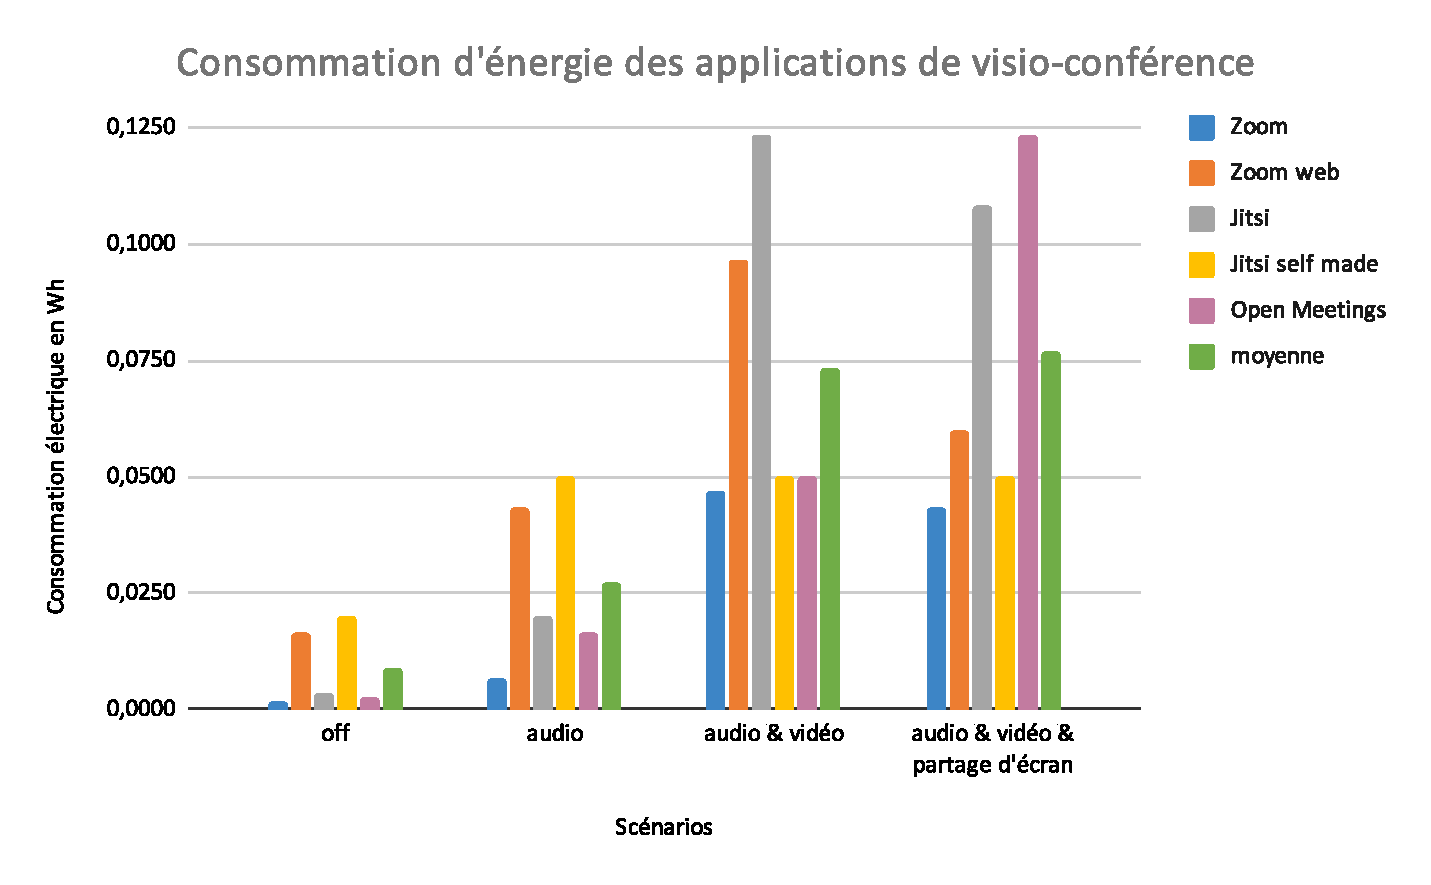
\includegraphics[width=1\linewidth]{graph_energie.pdf}
  \caption{Consommation d'énergie d'une minute de visioconférence}
  \label{fig:graph_energie}
\end{figure}

On peut remarquer que généralement l'utilisation de l'audio et la vidéo ainsi que le partage d'écran sont nettement plus énergivores que l'audio simple ou encore la connexion à la réunion sans intéractions. En effet, les réunion avec vidéo et audio sont en moyenne trois fois plus gourmande en énergie que les réunions ne faisant appel qu'à l'audio.

De plus, nous avons remarqué que même si les applications consomment 2 fois moins d'énergie en moyenne en mode off (sans aucun échange) que si l'audio est activé. Cependant, consommer de l'énergie pour ne rien faire est du gaspillage pur et dur.

Là où les applications Open Meetings et Jitsi (avec notre serveur hebergé sur l'ordinateur de Damien) sont plus performantes en audio, elles le deviennent beaucoup moins que les autres lorsque l'on active la vidéo, avec ou sans partage d'écran.

Enfin, on remarque  que Zoom reste l'application la plus performante peu importe le mode d'utilisation, au niveau de la consommation électrique c'est donc l'outil de visioconférence à privilégier. La pire étant en moyenne Jitsi (avec les serveurs de Jitsi).

\br L'ajout d'un partage d'écran dans une conférence audio et vidéo entraîne une baisse de la consommation énergétique dans toutes les applications excepté Openmeetings.

\noindent Ceci est dû notamment à l'affichage d'une seule vidéo sur l'interface des applications ainsi que du partage d'écran. Les vidéos des autres participants ne sont donc plus affichées par défaut.

\noindent Ceci n'explique néanmoins pas le cas d'Openmeetings... \eb 

\section{Données échangées des applications de visioconférence}

Dans ce paragraphe, nous allons nous intéréssser aux données échangées des applications de visioconférence entre l'ordinateur de l'utilisateur et le serveur. Comme précédemment, ces valeurs sont données pour une minute de visioconférence à 3 participants (mesure de 30 minutes normalisée à 1 minute). Plus la quantité de données est faible, plus l'impact environnemental de l'applcation est faible.

\begin{figure}[h]
  \centering
  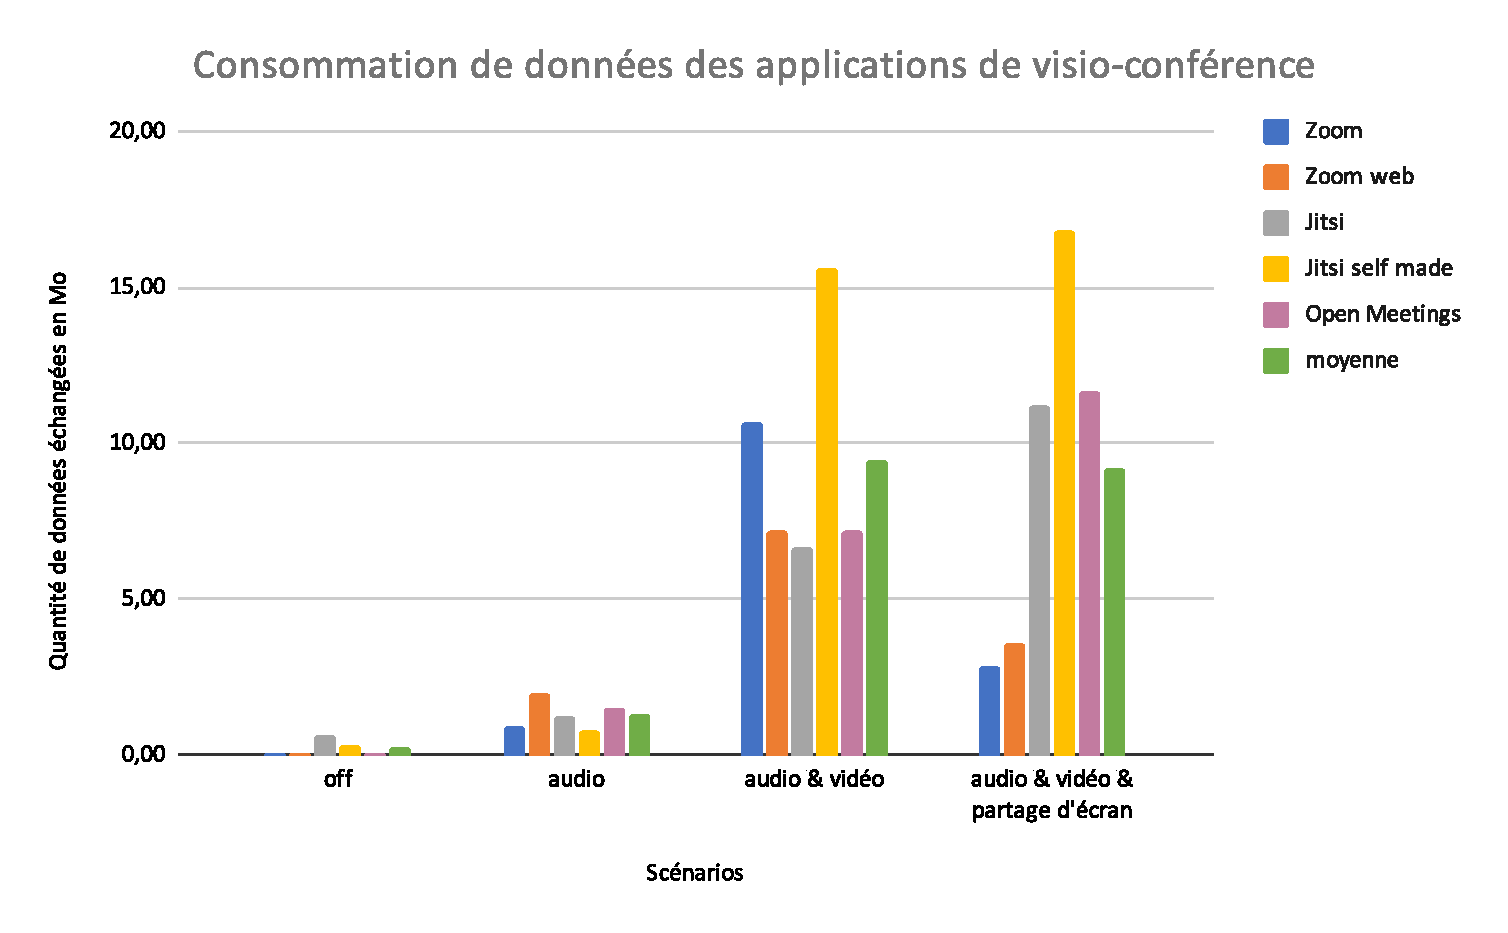
\includegraphics[width=1\linewidth]{graph_donnees.pdf}
  \caption{Consommation de données d'une minute de visioconférence}
  \label{fig:graph_donne}
\end{figure}

Comme montré sur la figure \ref{fig:graph_donne}, une minute de visioconférence en audio nécessite, en moyenne, 7 fois moins de données échangées qu’avec les caméras activées. Cependant, l'utilisation du partage d'écran est moins impactante que la vidéo. Son impact est, sur la moyenne des différentes mesures réalisées sur les applications de visioconférence, presque négligeable.

On peut également remarquer que lorsqu'aucune fonctionnalité de l'application n'est utilisée, la quantité de données échangée avec le serveur est certes faible mais non nulle. Ainsi, le simple fait de rester connecté sur l'application a un impact. 

Ensuite, aucune application ne semble plus performante en matière d'échange de données. Tout dépend du contexte d'utilisation. Zoom (sur l'application et le web) est la plus intéressante lorsqu'il s'agit d'utiliser la caméra, l'audio et le partage d'écran. Cependant lorsque l'audio et la caméra sont activés, les applications les plus intéressantes semblent être open-meeting et jitsi.  Pour le cas d'utilisation ne faisant intervenir que l'audio, toutes les solutions semblent être plus ou moins équivalentes même si Zoom et Jitsi semblent être plus performants dans ce cas.

\br L'ajout d'un partage d'écran dans une conférence audio et vidéo entraîne une baisse drastique de la consommation de données sur l'application Zoom. Comme dans le cas de la consommation énergétique, ceci est du au rendu d'une seule vidéo, ce qui réduit les données à transférer. 

\noindent Cependant, la baisse étant drastique, cela montre également une optimisation poussée de ce mode sur l'application. \eb 

\section{Impact carbone des applications de visioconférence (gEqCO2)}

Dans cette partie, nous avons réalisé la moyenne, pour tous les scénarios étudiés, de l'impact carbone  des applications en gEqCO2. Les résultats de cette étude sont présenté sur la figure \ref{fig:my_label}. Plus l'impact en carbone est faible, plus l'application est efficiente.

\begin{figure}[!h]
    \centering
    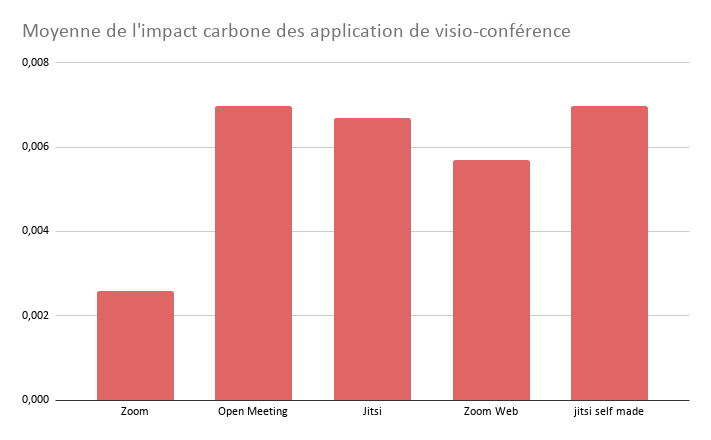
\includegraphics[scale=0.5]{moyenne.png}
    \caption{Impact moyen d'une application de visioconférence en gEqCO2}
    \label{fig:my_label}
\end{figure}

Comme nous l'avions prévu, c'est Zoom qui l'emporte largement devant les autres, avec une faible consommation électrique peu importe le cas d'utilisation et un échange de données entre le serveur et l'utilisateur plutôt bien géré. Or, Zoom est utilisé dans ce contexte avec l'application pour pc et mac. Son homologue sur web est quand à lui dans la moyenne des autres applications (également sur le web). Ainsi, utiliser l'application plutôt que la version web est (tout du moins pour zoom) une solution moins impactante en matière d'impact carbone.

\section{Du côté serveur}
Nous avons enregistré à l'aide de Scaphandre du côté du serveur Jitsi une puissance moyenne de 4,7 W pour les scénarios off et audio uniquement et une puissance moyenne de 5,5 W pour les scénarios vidéos et vidéos+partage d'écran. 

Ainsi, du côté serveur, l'avantage d'une conférence audio mais sans vidéo est encore une fois montré, même s'il faut recontextualiser ces valeurs au vu de la faible différence entre ces deux scénarios et du fait que le serveur hébergeant Jitsi est un ordinateur portable avec un processeur à basse consommation. Sur une baie de serveurs, le différence peut être plus importante, mais difficile à mesurer, car nous n'avons bien sûr pas accès aux serveurs Jitsi ou Zoom.

\section{Limites}

La précision des mesures que nous avons réalisées est conditionnée à la précision des outils de mesure utilisés. L'outil Carbonalyser propose effectivement une approximation de l'impact carbone. De même, les mesures effectuées par Scaphandre sont également une approximation de la consommation d'une machine. 

Ainsi, ces résultats sont à prendre dans le contexte d'une conférence de taille raisonnable et ne sont pas forcément transposables dans le cas d'une plus grande conférence où le besoin de serveurs mieux dimensionnés rendrait la consommation électrique ainsi que la consommation de données beaucoup plus élevés. Les différences entre scénarios seraient alors exacerbées à mesure que le nombre de participants ainsi que la taille des serveurs augmente.

\chapter*{Conclusion}
\addcontentsline{toc}{chapter}{Conclusion}

En définitive, notre étude a démontré qu'il était préférable de favoriser l’audio uniquement lors de vos réunions : le flux vidéo (caméra) aura tendance à consommer beaucoup plus. De plus, ajouter un partage d’écran n’est pas trop pénalisant s’il est utile.

Enfin, il est important de souligner qu'une réunion, même si aucun intervenant ne participe, est énergivore. Pensez donc a vous déconnecter si la réunion est finie. Enfin, n'hésitez pas à installer l'application pc ou mac de votre système de visioconférence préféré, votre impact carbone sera moindre et vous y aurez accès plus facilement.


\begin{thebibliography}{9}
\addcontentsline{toc}{chapter}{Bibliographie}
\bibitem{Greenspector} 
Kimberley DERUDDER, \textit{Quelle application mobile de visioconférence pour réduire votre impact ?}, Étude de Greenspector, 2020 [consulté le 1er avril 2021]

\url{https://greenspector.com/fr/quelle-application-mobile-de-visioconference-pour-reduire-votre-impact/}

\bibitem{UTC} 
Aurélien Béranger, Clément Brizard, Valentin Le Gauche, Yacine Baouch. \textit{Proposition d’une méthode d'évaluation environnementale multicritère des réunions en présentiel et en visio-conférence}, Rapport de l'UTC, 8 décembre 2020

\url{https://halshs.archives-ouvertes.fr/halshs-03120479/document}

\bibitem{Carbonalyser} 
The Shift Project, Présentation complète de Carbonalyser

\url{https://theshiftproject.org/carbonalyser-extension-navigateur}

\bibitem{Scaphandre} 
Documentation et sources de Scaphandre

\url{https://github.com/hubblo-org/scaphandre/}

\bibitem{Jitsi}
Documentation sur Jitsi

\url{https://jitsi.github.io/handbook/docs/devops-guide/devops-guide-quickstart}


\end{thebibliography}
\end{document}
